\documentclass[12pt, titlepage]{article}

\usepackage{fullpage}
\usepackage[round]{natbib}
\usepackage{multirow}
\usepackage{booktabs}
\usepackage{tabularx}
\usepackage{graphicx}
\usepackage{float}
\usepackage{hyperref}
\usepackage[normalem]{ulem} % for strikethrough
\hypersetup{
    colorlinks,
    citecolor=blue,
    filecolor=black,
    linkcolor=red,
    urlcolor=blue
}
\usepackage{longtable}


\input{../../Comments}
%% Common Parts

\newcommand{\progname}{Industrial Plant Designer} % PUT YOUR PROGRAM NAME HERE
\newcommand{\authname}{Team 18, Chemware Engineering
\\ Kishor Pandya
\\ Dhrumil Pandya
\\ Madhu Sivapragasam
\\ Rasik Pokharel} % AUTHOR NAMES                  

\usepackage{hyperref}
    \hypersetup{colorlinks=true, linkcolor=blue, citecolor=blue, filecolor=blue,
                urlcolor=blue, unicode=false}
    \urlstyle{same}
                                


\newcounter{acnum}
\newcommand{\actheacnum}{AC\theacnum}
\newcommand{\acref}[1]{AC\ref{#1}}

\newcounter{ucnum}
\newcommand{\uctheucnum}{UC\theucnum}
\newcommand{\uref}[1]{UC\ref{#1}}

\newcounter{mnum}
\newcommand{\mthemnum}{M\themnum}
\newcommand{\mref}[1]{M\ref{#1}}

\begin{document}

\title{Module Guide for \progname{}} 
\author{\authname}
\date{\today}

\maketitle

\pagenumbering{roman}

\section{Revision History}

\begin{tabularx}{\textwidth}{p{3cm}p{2cm}X}
  \toprule
  {\bf Date} & {\bf Version} & {\bf Notes} \\
  \midrule
  Jan 5th 2025 & 1.0 & Madhu Sivapragasam: Added auth and restore module definitions \\
  Jan 6th 2025 & 1.0 & Dhrumil Pandya: Added save and system data module definitions \\
  Jan 6th 2025 & 1.0 & Madhu Sivapragasam: Added timeline and module hierarchy sections \\
  Jan 6th 2025 & 1.1 & Kishor Pandya: Added user data and dashboard module definitions \\
  Jan 8th 2025 & 1.1 & Kishor Pandya: Added user interface and connection between req and design sections \\
  Jan 13th 2025 & 1.2 & Dhrumil Pandya: Added Design of Communication Protocols section and use hierarchy between modules section \\
  Jan 13th 2025 & 1.2 & Rasik Pokharel: Added canvas module and anticipated changes \\
  Jan 16th 2025 & 1.3 & Madhu Sivapragasam: Add traceability matrix between requirements and modules \\
  Jan 16th 2025 & 1.3 & Madhu Sivapragasam: Add Simulation module \\
  Jan 16th 2025 & 1.4 & Rasik Pokharel: Add traceability matrix between AC modules \\
  \textcolor{blue}{April 3rd 2025} & \textcolor{blue}{2.0} & \textcolor{blue}{Madhu Sivapragasam: Small changes for rev 1} \\
  \bottomrule
  \end{tabularx}
  

\newpage

\section{Reference Material}

This section records information for easy reference.

\subsection{Abbreviations and Acronyms}

\renewcommand{\arraystretch}{1.2}
\begin{tabular}{l l} 
  \toprule		
  \textbf{symbol} & \textbf{description}\\
  \midrule 
  AC & Anticipated Change\\
  DAG & Directed Acyclic Graph \\
  M & Module \\
  MG & Module Guide \\
  OS & Operating System \\
  R & Requirement\\
  SC & Scientific Computing \\
  SRS & Software Requirements Specification\\
  \progname & Name of the factory simulation software that is being developed\\
  UC & Unlikely Change \\
  \bottomrule
\end{tabular}\\

\newpage

\tableofcontents

\listoftables

\listoffigures

\newpage

\pagenumbering{arabic}

\section{Introduction}

Decomposing a system into modules is a commonly accepted approach to developing
software.  A module is a work assignment for a programmer or programming
team~\citep{ParnasEtAl1984}.  We advocate a decomposition
based on the principle of information hiding~\citep{Parnas1972a}.  This
principle supports design for change, because the ``secrets'' that each module
hides represent likely future changes.  Design for change is valuable in SC,
where modifications are frequent, especially during initial development as the
solution space is explored.  

Our design follows the rules layed out by \citet{ParnasEtAl1984}, as follows:
\begin{itemize}
\item System details that are likely to change independently should be the
  secrets of separate modules.
\item Each data structure is implemented in only one module.
\item Any other program that requires information stored in a module's data
  structures must obtain it by calling access programs belonging to that module.
\end{itemize}

After completing the first stage of the design, the Software Requirements
Specification (SRS), the Module Guide (MG) is developed~\citep{ParnasEtAl1984}. The MG
specifies the modular structure of the system and is intended to allow both
designers and maintainers to easily identify the parts of the software.  The
potential readers of this document are as follows:

\begin{itemize}
\item New project members: This document can be a guide for a new project member
  to easily understand the overall structure and quickly find the
  relevant modules they are searching for.
\item Maintainers: The hierarchical structure of the module guide improves the
  maintainers' understanding when they need to make changes to the system. It is
  important for a maintainer to update the relevant sections of the document
  after changes have been made.
\item Designers: Once the module guide has been written, it can be used to
  check for consistency, feasibility, and flexibility. Designers can verify the
  system in various ways, such as consistency among modules, feasibility of the
  decomposition, and flexibility of the design.
\end{itemize}

The rest of the document is organized as follows. Section
\ref{SecChange} lists the anticipated and unlikely changes of the software
requirements. Section \ref{SecMH} summarizes the module decomposition that
was constructed according to the likely changes. Section \ref{SecConnection}
specifies the connections between the software requirements and the
modules. Section \ref{SecMD} gives a detailed description of the
modules. Section \ref{SecTM} includes two traceability matrices. One checks
the completeness of the design against the requirements provided in the SRS. The
other shows the relation between anticipated changes and the modules. Section
\ref{SecUse} describes the use relation between modules.

\section{Anticipated and Unlikely Changes} \label{SecChange}

This section lists possible changes to the system. According to the likeliness
of the change, the possible changes are classified into two
categories. Anticipated changes are listed in Section \ref{SecAchange}, and
unlikely changes are listed in Section \ref{SecUchange}.

\textcolor{blue}{These anticipated and unlikely changes still apply even after the completion of revision 1 since the project is being passed over to another team. For that new teams work they will still need to consider the reason and impact for these changes and so rather than remove the changes we have chosen to continue listing them below.}

\subsection{Anticipated Changes} \label{SecAchange}

Anticipated changes are the source of the information that is to be hidden
inside the modules. Ideally, changing one of the anticipated changes will only
require changing the one module that hides the associated decision. The approach
adapted here is called design for
change.



\begin{description}


    \item [\refstepcounter{acnum} \actheacnum \label{acUserInterface}:]User Interface Updates:
    \begin{itemize}
        \item \textbf{Reason:} Users may request a more intuitive or visually appealing interface. These changes are anticipated to resemble existing market solutions.
        \item \textbf{Impact:} Modifications to the Canvas Module to enhance features or improve visualization.
    \end{itemize}

    \item [\refstepcounter{acnum} \actheacnum \label{acAuth}:]Authentication Mechanism Enhancements:
    \begin{itemize}
        \item \textbf{Reason:} As security needs evolve, requiring stricter authentication methods stricter methods may become required. Multi-factored authentication is anticipated.
        \item \textbf{Impact:} Updates to the Authentication Module to support new security frameworks and facilitate more users. 
    \end{itemize}

    \item [\refstepcounter{acnum} \actheacnum \label{acAuth}:] Integration with New Data Sources:
    \begin{itemize}
        \item \textbf{Reason:} As the system functionality is expanded to include more data sources for simulation and visualization new data integrations are expected.
        
        \item \textbf{Impact:} Changes to the System Data Module or User Data Module to handle new data. 
    \end{itemize}

    \item  [\refstepcounter{acnum} \actheacnum \label{acAuth}:]Scaling Requirements:
    \begin{itemize}
        \item \textbf{Reason:} As the system increases, the performance of the system does as well. Especially given the expected increase in concurrent users, performance optimization will be a key piece in scaling the system.
        \item \textbf{Impact:} Optimization of all the data modules M3-M7 and M9 to handle larger datasets efficiently.
    \end{itemize}


    \item  [\refstepcounter{acnum} \actheacnum \label{acAuth}:]New Features or Functionalities:
    \begin{itemize}
        \item \textbf{Reason:} As the implementation timeline gets closer, the users of the system push for features and functionalities that they didn't initially anticipate.
      
        \item \textbf{Impact:} Updates to all the behavior-hiding modules may be required to incorporate new features.
    \end{itemize}

    \item  [\refstepcounter{acnum} \actheacnum \label{acAuth}:]Dependency Updates:
    \begin{itemize}
        \item \textbf{Reason:} Any dependencies such as react libraries that were used in the creation of existing modules are subject to change. 
        \item \textbf{Impact:} Canvas, Save and Restore, Dashboard could all be impacted.
    \end{itemize}

    \item  [\refstepcounter{acnum} \actheacnum \label{acAuth}:]System-Wide Performance Improvements:
    \begin{itemize}
        \item \textbf{Reason:} The need to reduce latency and optimize system response times, especially optimizing simulation script interfacing.
        \item \textbf{Impact:} Refactoring of modules such as System Data Module or Save Module to optimize routing and database queries.
    \end{itemize}

        \item [\refstepcounter{acnum} \actheacnum \label{acAuth}:] Hardware of the system:
    \begin{itemize}
        \item \textbf{Reason:} Changes in hosting decisions could change the hardware and underlying OS of the systems involved.
        \item \textbf{Impact:} M1 Hardware hiding modules will be impacted by this change. 
    \end{itemize}

\end{description}




\subsection{Unlikely Changes} \label{SecUchange}

The module design should be as general as possible. However, a general system is
more complex. Sometimes this complexity is not necessary. Fixing some design
decisions at the system architecture stage can simplify the software design. If
these decisions should later need to be changed, then many parts of the design
will potentially need to be modified. Hence, it is not intended that these
decisions will be changed.

\begin{description}


\item[\refstepcounter{ucnum} \uctheucnum \label{ucCoreData}:] Core Data Structure Changes:
  \begin{itemize}
    \item \textbf{Reason:} The system is built on specific data structures optimized for its operations that will not be subject to change. These changes are not likely to occur as they've been thoroughly finalized. 
    \item \textbf{Impact:} Changing these core data structures would require significant architectural changes.
  \end{itemize}

\item[\refstepcounter{ucnum} \uctheucnum \label{ucAuth}:] Removal of any existing features:
  \begin{itemize}
    \item \textbf{Reason:} The system is being built from the base up, all existing features will remain.
    \item \textbf{Impact:} Features are being built on top of each other, removing any existing core feature could be breaking change.
  \end{itemize}

\item[\refstepcounter{ucnum} \uctheucnum \label{ucModular}:] Removal of Modular Design:
  \begin{itemize}
    \item \textbf{Reason:} The modular structure is fundamental to the system's scalability and maintainability.
    \item \textbf{Impact:} Transitioning to a monolithic architecture would require significant rework and is unlikely given the benefits of modular design.
  \end{itemize}

\item[\refstepcounter{ucnum} \uctheucnum \label{ucLanguage}:] System Language Change:
  \begin{itemize}
    \item \textbf{Reason:} The system language has been thoroughly thought about and decided upon.
    \item \textbf{Impact:} Changing the primary language would require rewriting all code, libraries, and integrations.
  \end{itemize}

\item[\refstepcounter{ucnum} \uctheucnum \label{ucAPI}:] Elimination of API Support:
  \begin{itemize}
    \item \textbf{Reason:} API integrations are crucial for the system to connect with external services and data sources.
    \item \textbf{Impact:} Removing API support would hinder functionality and require redesigning the System Data Module and User data module.
  \end{itemize}

\end{description}




\section{Module Hierarchy} \label{SecMH}

This section provides an overview of the module design. Modules are summarized
in a hierarchy decomposed by secrets in Table \ref{TblMH}. The modules listed
below, which are leaves in the hierarchy tree, are the modules that will
actually be implemented.

\begin{description}
\item [\refstepcounter{mnum} \mthemnum \label{mHH}:] Hardware-Hiding Module
\item [\refstepcounter{mnum} \mthemnum \label{mAuth}:] Authentication Module
\item [\refstepcounter{mnum} \mthemnum \label{mSave}:] Save Module
\item [\refstepcounter{mnum} \mthemnum \label{mRestore}:] Restore Module
\item [\refstepcounter{mnum} \mthemnum \label{mCanvas}:] Canvas Module
\item [\refstepcounter{mnum} \mthemnum \label{mSystem}:] System Data Module
\item [\refstepcounter{mnum} \mthemnum \label{mUser}:] User Data Module
\item [\refstepcounter{mnum} \mthemnum \label{mDashboard}:] Dashboard Module
\item [\refstepcounter{mnum} \mthemnum \label{mSimulation}:] Simulation Module
\end{description}


\begin{table}[h!]
\centering
\begin{tabular}{p{0.3\textwidth} p{0.6\textwidth}}
\toprule
\textbf{Level 1} & \textbf{Level 2}\\
\midrule

{Hardware-Hiding Module} & \mref{mHH} \\
\midrule

\multirow{7}{0.3\textwidth}{Behaviour-Hiding Module} & \mref{mAuth}\\
& \mref{mSave}\\
& \mref{mRestore}\\
& \mref{mCanvas}\\
& \mref{mSystem}\\
& \mref{mUser}\\
& \mref{mDashboard}\\

\midrule

\multirow{1}{0.3\textwidth}{Software Decision Module} & \mref{mSimulation}\\

\bottomrule

\end{tabular}
\caption{Module Hierarchy}
\label{TblMH}
\end{table}

\section{Connection Between Requirements and Design} \label{SecConnection}

The design of the system is intended to satisfy the requirements developed in
the SRS. In this stage, the system is decomposed into modules. The connection
between requirements and modules is listed in Table~\ref{TblRT}.

\section{Module Decomposition} \label{SecMD}

Modules are decomposed according to the principle of ``information hiding''
proposed by \citet{ParnasEtAl1984}. The \emph{Secrets} field in a module
decomposition is a brief statement of the design decision hidden by the
module. The \emph{Services} field specifies \emph{what} the module will do
without documenting \emph{how} to do it. For each module, a suggestion for the
implementing software is given under the \emph{Implemented By} title. If the
entry is \emph{OS}, this means that the module is provided by the operating
system or by standard programming language libraries.  \emph{\progname{}} means the
module will be implemented by the \progname{} software.

Only the leaf modules in the hierarchy have to be implemented. If a dash
(\emph{--}) is shown, this means that the module is not a leaf and will not have
to be implemented.

\subsection{Hardware Hiding Modules (\mref{mHH})}

\begin{description}
\item[Secrets:]The data structure and algorithm used to implement the virtual
  hardware.
\item[Services:]Serves as a virtual hardware used by the rest of the
  system. This module provides the interface between the hardware and the
  software. So, the system can use it to display outputs or to accept inputs.
\item[Implemented By:] OS
\end{description}

\subsection{Behaviour-Hiding Module}

\begin{description}
  \item[Secrets:]The contents of the required behaviours.
  \item[Services:]Includes programs that provide externally visible behaviour of
    the system as specified in the software requirements specification (SRS)
    documents. This module serves as a communication layer between the
    hardware-hiding module and the software decision module. The programs in this
    module will need to change if there are changes in the SRS.
  \item[Implemented By:] --
\end{description}

\subsubsection{Authentication Module (\mref{mAuth})}

\begin{description}
\item[Secrets:]The methods for handling authentication of users into the application
\item[Services:]Enables users to register an account, login to their account and validates all requests made by the user to the API modules
\item[Implemented By:] [\progname]
\item[Type of Module:] [Abstract Object]
\end{description}

\subsubsection{Restore Module (\mref{mRestore})}
\begin{description}
\item[Secrets:]The method for recovering previously built diagrams 
\item[Services:]Provides a list of previously developed diagrams and enables diagram data to be loaded into the canvas module
\item[Implemented By:] [\progname]
\item[Type of Module:] [Library]
\end{description}

\subsubsection{Save Module (\mref{mSave})}
\begin{description}
\item[Secrets:] The process of storing and updating diagrams (including domain snapshots) into the user database.
\item[Services:] Provides creation and update endpoints for saving diagrams, canvas data, and domain snapshots.
\item[Implemented By:] [\progname]
\item[Type of Module:] [Library]
\end{description}

\subsubsection{System Data Module (\mref{mSystem})}
\begin{description}
\item[Secrets:] The underlying routing and request-handling logic to interact with the system data.
\item[Services:] Exposes GET HTTP routes for domain data retrieval.
\item[Implemented By:] [\progname]
\item[Type of Module:] [Abstract Object]
\end{description}

\subsubsection{User Data Module (\mref{mUser})}
\begin{description}
\item[Secrets:] The underlying routing and request-handling logic to interact with the user data.
\item[Services:] Exposes GET, POST, and PUT HTTP routes for user data manipulation.
\item[Implemented By:] [\progname]
\item[Type of Module:] [Abstract Object]
\end{description}

\subsubsection{Dashboard Module (\mref{mDashboard})}
\begin{description}
\item[Secrets:]The methods for handling users choose between creating new canvas or loading an existing one.
\item[Services:]Provides a list of previously developed diagrams and/or enables a new canvas module to be created.
\item[Implemented By:] [\progname]
\item[Type of Module:] [Library]
\end{description}

\subsubsection{Canvas Module (\mref{mCanvas})}
\begin{description}
\item[Secrets:] The underlying logic for data-driven nodes and edges. 
\item[Services:] Displays the nodes and edges to the screen displaying data provided by various data modules. Allows users to interact with system data in each node and edge. Users can drag and drop, reshape, move the canvas, and perform other manipulations. Implements node and edge core functionalities using the React library "React Flow.
\item[Implemented By:] [\progname]
\item[Type of Module:] [Abstract Object]
\end{description}

\subsection{Software Decision Module}

\begin{description}
\item[Secrets:] The design decision based on mathematical theorems, physical
  facts, or programming considerations. The secrets of this module are
  \emph{not} described in the SRS.
\item[Services:] Includes data structure and algorithms used in the system that
  do not provide direct interaction with the user. 
  % Changes in these modules are more likely to be motivated by a desire to
  % improve performance than by externally imposed changes.
\item[Implemented By:] --
\end{description}

\subsubsection{Simulation Module (\mref{mSimulation})}
\begin{description}
\item[Secrets:] The model that computes the outputs of the factory system based off of the inputs 
\item[Services:] Computes output data for the factory using an internal algorithm and the provided inputs. 
\item[Implemented By:] Professor Mahelec (capstone sponsor)
\item[Type of Module:] [Library]
\end{description}

\section{Traceability Matrix} \label{SecTM}

This section shows two traceability matrices: between the modules and the
requirements and between the modules and the anticipated changes.

% the table should use mref, the requirements should be named, use something
% like fref
\renewcommand{\arraystretch}{1.2} % Optional: Adjusts row spacing
\begin{longtable}{p{0.2\textwidth} p{0.6\textwidth}}
\toprule
\textbf{Req.} & \textbf{Modules} \\
\midrule
\endfirsthead
\toprule
\textbf{Req.} & \textbf{Modules} \\
\midrule
\endhead
\midrule
\multicolumn{2}{r}{\textit{Continued on next page...}} \\
\midrule
\endfoot
\bottomrule
\endlastfoot
FR1 & \mref{mCanvas}, \mref{mSystem} \\
FR2 & \mref{mCanvas}, \mref{mSystem} \\
FR3 & \mref{mSimulation} \\
FR4 & \mref{mCanvas}, \mref{mSave} \\
FR5 & \mref{mAuth}, \mref{mSave}. \mref{mUser} \\
FR6 & \mref{mAuth}, \mref{mRestore}, \mref{mUser}, \mref{mDashboard} \\
FR7 & \mref{mCanvas} \\
FR8 & \mref{mRestore}, \mref{mDashboard} \\
FR9 & \mref{mSave}, \mref{mCanvas}, \mref{mUser} \\
FR10 & \mref{mCanvas} \\
LAFAR1 & \mref{mCanvas}\\
LAFAR2 & \mref{mCanvas}, \mref{mDashboard}\\
LAFAR3 & \mref{mCanvas}\\
LAFSR1 & \mref{mCanvas}, \mref{mDashboard}\\
LAFSR2 & \mref{mCanvas}, \mref{mDashboard}\\
LAFSR3 & \mref{mCanvas}, \mref{mDashboard}\\
UHE1 & \mref{mCanvas}, \mref{mDashboard}\\
UHE2 & \mref{mCanvas}, \mref{mDashboard}\\
UHPI1 & \mref{mCanvas}, \mref{mDashboard}\\
UHL1 & All modules\\
UHL2 & \mref{mCanvas}, \mref{mDashboard}\\
UHU1 & \mref{mSystem}, \mref{mCanvas}, \mref{mDashboard}\\
UHA1 & \mref{mHH}\\
PS1 & \mref{mCanvas}, \mref{mDashboard}\\
PS2 & \mref{mSave}\\
PS3 & \mref{mRestore}\\
PS4 & \mref{mSimulation}\\
PPA1 & \mref{mSimulation}, \mref{mCanvas}\\
PPA2 & \mref{mCanvas}\\
PRF1 & \mref{mSimulation}\\
PRF2 & \mref{mCanvas}, \mref{mSystem}, \mref{mSave} \\
PC1 & \mref{mUser}, \mref{mCanvas}, \mref{mSave}, \mref{mRestore}\\
PSE1 & All modules\\
PL1 & All modules\\
OEEP1 & \mref{mHH}\\
OEEP2 & All modules\\
OEEP3 & \mref{mHH}\\
OEWE1 & \mref{mAuth}, \mref{mSave}, \mref{mRestore}\\
OEWE2 & \mref{mUser}, \mref{mSystem}\\
OEIA1 & \mref{mRestore}, \mref{mDashboard}\\
OEIA2 & \mref{mSimulation}\\
OEP1 & All modules\\
OER1 & All modules\\
MSM1 & All modules\\
MSM2 & All modules\\
MSS1 & All modules\\
MSA1 & All modules\\
MSA2 & All modules\\
\textcolor{blue}{\sout{SEC-ACC1}} & \textcolor{blue}{\sout{\mref{mAuth}}}\\
SEC-INT1 & \mref{mCanvas}, \mref{mSave}\\
SEC-INT2 & \mref{mAuth}, \mref{mUser}, \mref{mSystem}\\
SEC-PRI1 & \mref{mAuth}, \mref{mUser}\\
SEC-AUD1 & \mref{mAuth}, \mref{mUser}\\
SEC-IMM1 & All modules\\
CR1 & All modules\\
LR1 & All modules\\
LR2 & All modules\\


\caption{Trace Between Requirements and Modules}
\label{TblRT}
% Continue adding rows as necessary...
\end{longtable}

\begin{table}[H]
\centering
\begin{tabular}{p{0.2\textwidth} p{0.6\textwidth}}
\toprule
\textbf{AC} & \textbf{Modules}\\
\midrule
AC1 & \mref{mCanvas}\\
AC2 & \mref{mAuth}\\
AC3 & \mref{mSystem}, \mref{mUser} \\
AC4 & \mref{mSystem}, \mref{mUser},\mref{mSave}, \mref{mRestore}, \mref{mSimulation} \\
AC5 & \mref{mAuth},\mref{mSystem}, \mref{mUser},\mref{mSave}, \mref{mRestore},\\
AC6 & \mref{mCanvas}, \mref{mSave}, \mref{mRestore}, \mref{mSave}, \mref{mDashboard}\\
AC7 & \mref{mSystem}, \mref{mSave}\\
AC8 & \mref{mHH}\\

\bottomrule
\end{tabular}
\caption{Trace Between Anticipated Changes and Modules}
\label{TblACT}
\end{table}

\section{Use Hierarchy Between Modules} \label{SecUse}

\begin{figure}[H]
\centering
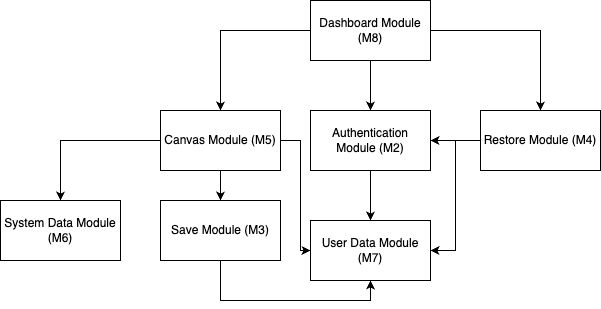
\includegraphics[width=0.7\textwidth]{use-hierarchy.png}
\caption{Use hierarchy among modules}
\label{FigUH}
\end{figure}

%\section*{References}

\section{User Interfaces}
The user interface of the app includes multiple screens, whose screenshots have been added in the appendix. You can also view the multiple screens on Figma through \href{https://www.figma.com/design/fCKXo1IHksfcUOUxzCmHca/Capstone?node-id=0-1&t=MoTPORPUNylEgVLm-1}{this link}.  

The user interface is designed to allow users ease of use and functionality. The authentication pages all have a simple UI easy for anyone to understand. The canvas page is designed to help users build plant models and be able to visualize the model and all its data in one place.  

\subsection*{Layout and Structure}
The UI follows a structured layout with clear divisions, likely employing grid-based design principles. The interface emphasizes simplicity and usability, ensuring content and interactive elements are accessible.  

\textbf{Header or Navigation Bar:} The top of the page may include navigation controls, such as menus or titles.  

\subsection*{Components}
\begin{itemize}
    \item \textbf{Buttons:} The interface includes clickable buttons, styled with rounded corners, clear labels, and hover effects. Buttons are functional for actions like submitting forms, navigating between sections, or initiating specific tasks.
    \item \textbf{Input Fields:} Text input fields are prominently displayed, designed for user interaction. Labels or placeholders guide users to enter the required data.
    \item \textbf{Interactive Widgets:} Dropdowns, checkboxes, or other selection tools are present to allow users to make choices. Sliders or toggles may allow for dynamic adjustments.
    \item \textbf{Modals or Pop-ups:} If the interface uses modals, they highlight additional information or options while keeping the background slightly dimmed.
    \item \textbf{Icons:} Relevant icons visually complement buttons or other actions, making the interface intuitive.
\end{itemize}  

\subsection*{Visual Design}
\begin{itemize}
    \item \textbf{Color Scheme:} A clean and professional palette is used, with contrasts for primary actions (e.g., a bright accent color for buttons). Background colors are neutral, ensuring readability.
    \item \textbf{Typography:} Fonts are consistent, with distinct styles for headings, subheadings, and body text. Adequate spacing is maintained to avoid clutter.
    \item \textbf{Spacing and Padding:} Generous padding and margins separate sections, enhancing readability and reducing cognitive load.
\end{itemize}  

\subsection*{Navigation and Interaction}
\begin{itemize}
    \item \textbf{Flow:} The design supports a step-by-step or task-oriented flow, guiding users through actions intuitively. Navigation elements (e.g., a sidebar or breadcrumbs) ensure seamless movement across sections.
    \item \textbf{Responsiveness:} The layout is adaptive, ensuring usability on multiple devices, though this can only be confirmed through testing.
\end{itemize}  

\subsection*{Purpose and Context}
The UI serves specific functions, such as:
\begin{itemize}
    \item Collecting user input or data.
    \item Displaying analytics, dashboards, or summaries.
    \item Providing actionable controls for workflows or applications.
\end{itemize}

\section{Design of Communication Protocols}

Our system implements a standard RESTful communication protocol over HTTP for all client--server interactions. Each module providing services (e.g., saving diagrams, restoring diagrams, retrieving system/domain data, user account creation, etc.) exposes one or more HTTP endpoints. All request and response bodies are encoded in JSON.

\subsection{Request--Response Model}

\begin{itemize}
    \item The frontend (Canvas and Dashboard modules in the browser) sends requests (e.g., \texttt{GET}, \texttt{POST}, \texttt{PUT}, \texttt{DELETE}) via Axios to the backend
    \item The server responds to each request with a JSON response indicating success or error states
\end{itemize}

\subsection{Authentication}

\begin{itemize}
    \item JWT (JSON Web Tokens) are used for stateless authentication
    \item Clients get a \texttt{refreshToken} upon successful login
    \item All subsequent API requests include the \texttt{accessToken} in the \texttt{Authorization} header (\texttt{Bearer <token>}) to authenticate
    \item The Authentication Module (\texttt{mAuth}) checks token validity and only allows authorized users to access or mutate the data
\end{itemize}

\subsection{Payload and Data Serialization}

\begin{itemize}
    \item Diagram data and domain snapshots are serialized as ``stringified'' JSON when sent to or stored in the database
    \item User data (email, password hashes, profile information) is similarly sent over HTTPS as JSON
\end{itemize}

\subsection{Status Code and Error Handling}

\begin{itemize}
    \item Standard HTTP status codes are used for different types of responses:
    \begin{itemize}
        \item \texttt{200 OK}
        \item \texttt{201 Created}
        \item \texttt{400 Bad Request}
        \item \texttt{401 Unauthorized}
        \item \texttt{403 Forbidden}
        \item \texttt{404 Not Found}
        \item \texttt{500 Internal Server Error}
    \end{itemize}
    \item Errors are returned in JSON format:
    \begin{verbatim}
    {
        "message": "Invalid credentials",
        "details": { ... }
    }
    \end{verbatim}
\end{itemize}

\subsection{Example Request and Response Structures}

In this section, we have outlined the example of a few requests and responses that can be made to the backend server.

\subsubsection{GET Request Example (Fetch Domain Data)}

\begin{verbatim}
Request:
GET /api/data/domain/{domainId}
Authorization: Bearer <accessToken>

Response (200 OK):
{
  "id": "d1234",
  "name": "ChemicalDomain",
  "models": [...],
  "streams": [...],
  "colors": [...]
}
\end{verbatim}

\noindent
The server returns a 404 error if the requested domain does not exist, e.g.:
\begin{verbatim}
Response (404 Not Found):
{
  "message": "Domain not found"
}
\end{verbatim}

\subsubsection{POST Request Example (Save a New Diagram)}

\begin{verbatim}
Request:
POST /api/data/diagrams
Authorization: Bearer <accessToken>
Content-Type: application/json

Body:
{
  "name": "MyFirstDiagram",
  "canvas": "{ \"nodes\": [...], \"edges\": [...], ... }",
  "parameters": "{ ... }",
  "domainId": "d1234",
  "snapshotData": { ... }
}

Response (201 Created):
{
  "message": "Diagram created successfully",
  "diagram": {
    "id": "diag5678",
    "name": "MyFirstDiagram",
    "canvas": "...",
    "parameters": "...",
    "snapshotId": "snap9999"
  }
}
\end{verbatim}

\noindent
If missing required fields, the server returns a 400 error, e.g.:
\begin{verbatim}
Response (400 Bad Request):
{
  "message": "Name, canvas, and parameters are required"
}
\end{verbatim}

\subsubsection{PUT Request Example (Update Existing Diagram)}

\begin{verbatim}
Request:
PUT /api/data/diagrams/{diagramId}
Authorization: Bearer <accessToken>
Content-Type: application/json

Body:
{
  "name": "UpdatedDiagram",
  "canvas": "{ \"nodes\": [...], \"edges\": [...], ... }",
  "parameters": "{ ... }",
  "updatedSnapshotData": { ... }
}

Response (200 OK):
{
  "message": "Diagram updated successfully",
  "diagram": {
    "id": "diag5678",
    "name": "UpdatedDiagram",
    "canvas": "...",
    "parameters": "..."
  }
}
\end{verbatim}

\noindent
A 403 Forbidden is returned if the user does not own the diagram.

\subsubsection{DELETE Request Example (Remove a Refresh Token)}

\begin{verbatim}
Request:
DELETE /api/auth/logout
Authorization: Bearer <refreshToken>

Response (200 OK):
{
  "message": "Logged out successfully"
}
\end{verbatim}

\noindent
The server deletes the associated refresh token from the database. If the token is invalid, a 403 error will be returned.

\section{Timeline}
The timeline for the development of each of the modules is displayed in the below table which includes module title, responsible developer(s) and the timeline in which the module was developed. The hardware hiding module (\mref{mHH}) is not being implemented and the simulation module (\mref{mSimulation}) is provided by the project sponsor and so they are not included in the timeline. 

\begin{table}[h!]
  \centering
  \begin{tabular}{|l|l|l|}
  \hline
  \textbf{Module Name} & \textbf{Responsible Developer(s)} & \textbf{Timeline} \\ \hline
  System Data Module (\mref{mSystem})      & Dhrumil Pandya              & Nov 2024 - Dec 2024     \\ \hline
  User Data Module (\mref{mUser}) & Kishor Padya                      & Nov 2024 - Dec 2024     \\ \hline
  Canvas Module (\mref{mCanvas})         & Madhu Sivapragasam, Rasik Pokharel          & Nov 2024 - Dec 2024        \\ \hline
  Dashboard Module (\mref{mDashboard})    & Rasik Pokharel                  & Dec 2024 - Jan 2025       \\ \hline
  Authentication module (\mref{mAuth})       & Kishor Pandya          & Dec 2024 - Jan 2025            \\ \hline
  Save Module (\mref{mSave})       & Madhu Sivapragasam         & Dec 2024 - Jan 2025             \\ \hline
  Restore Module (\mref{mSave})       & Dhrumil Pandya       & Dec 2024 - Jan 2025             \\ \hline
  \end{tabular}
  \caption{Development Timelome}
  \label{tab:modules}
  \end{table}

The month of February will be reserved for module testing where the developers responsible for each module will test and verify the performance of their respective modules. This will be done through manual testing as well as automated test suites. Any errors or bugs will also be fixed during this time period. 

\section{Appendix}
This section includes the screenshots of the app's user interface, along with descriptive titles for each screen.

\begin{figure}[H]
    \centering
    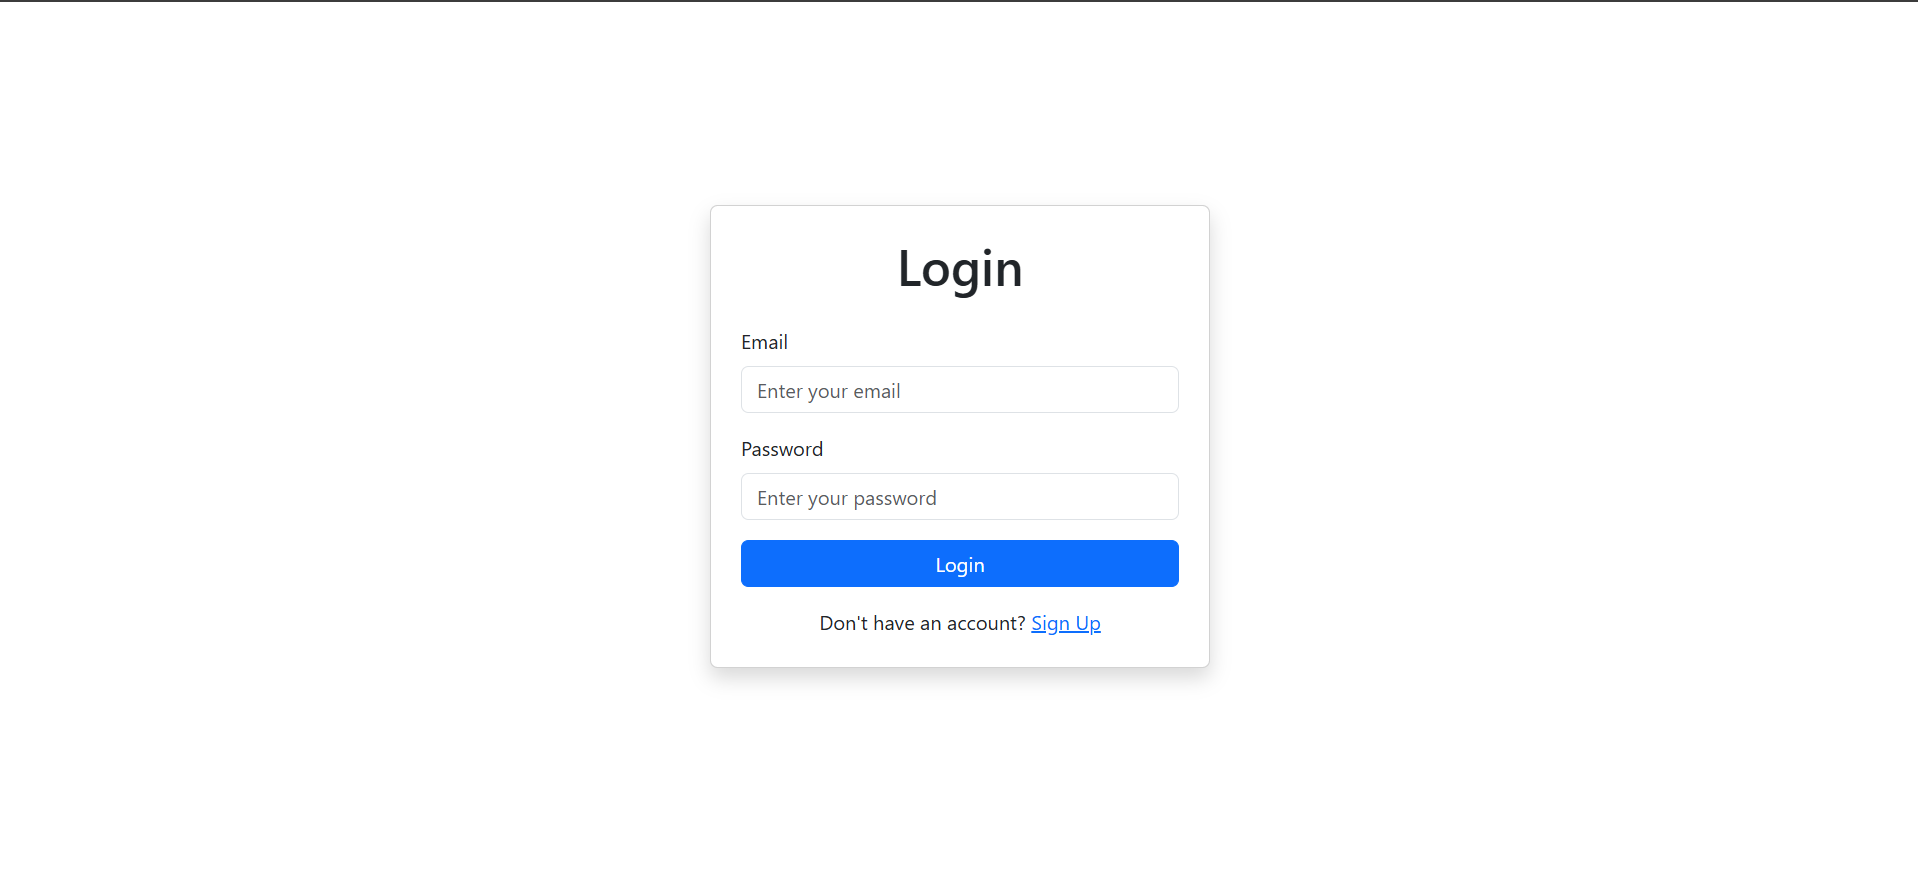
\includegraphics[width=\textwidth]{./UI_images/Login.png}
    \caption{Login Page}
    \label{fig:auth_page}
\end{figure}

\begin{figure}[H]
  \centering
  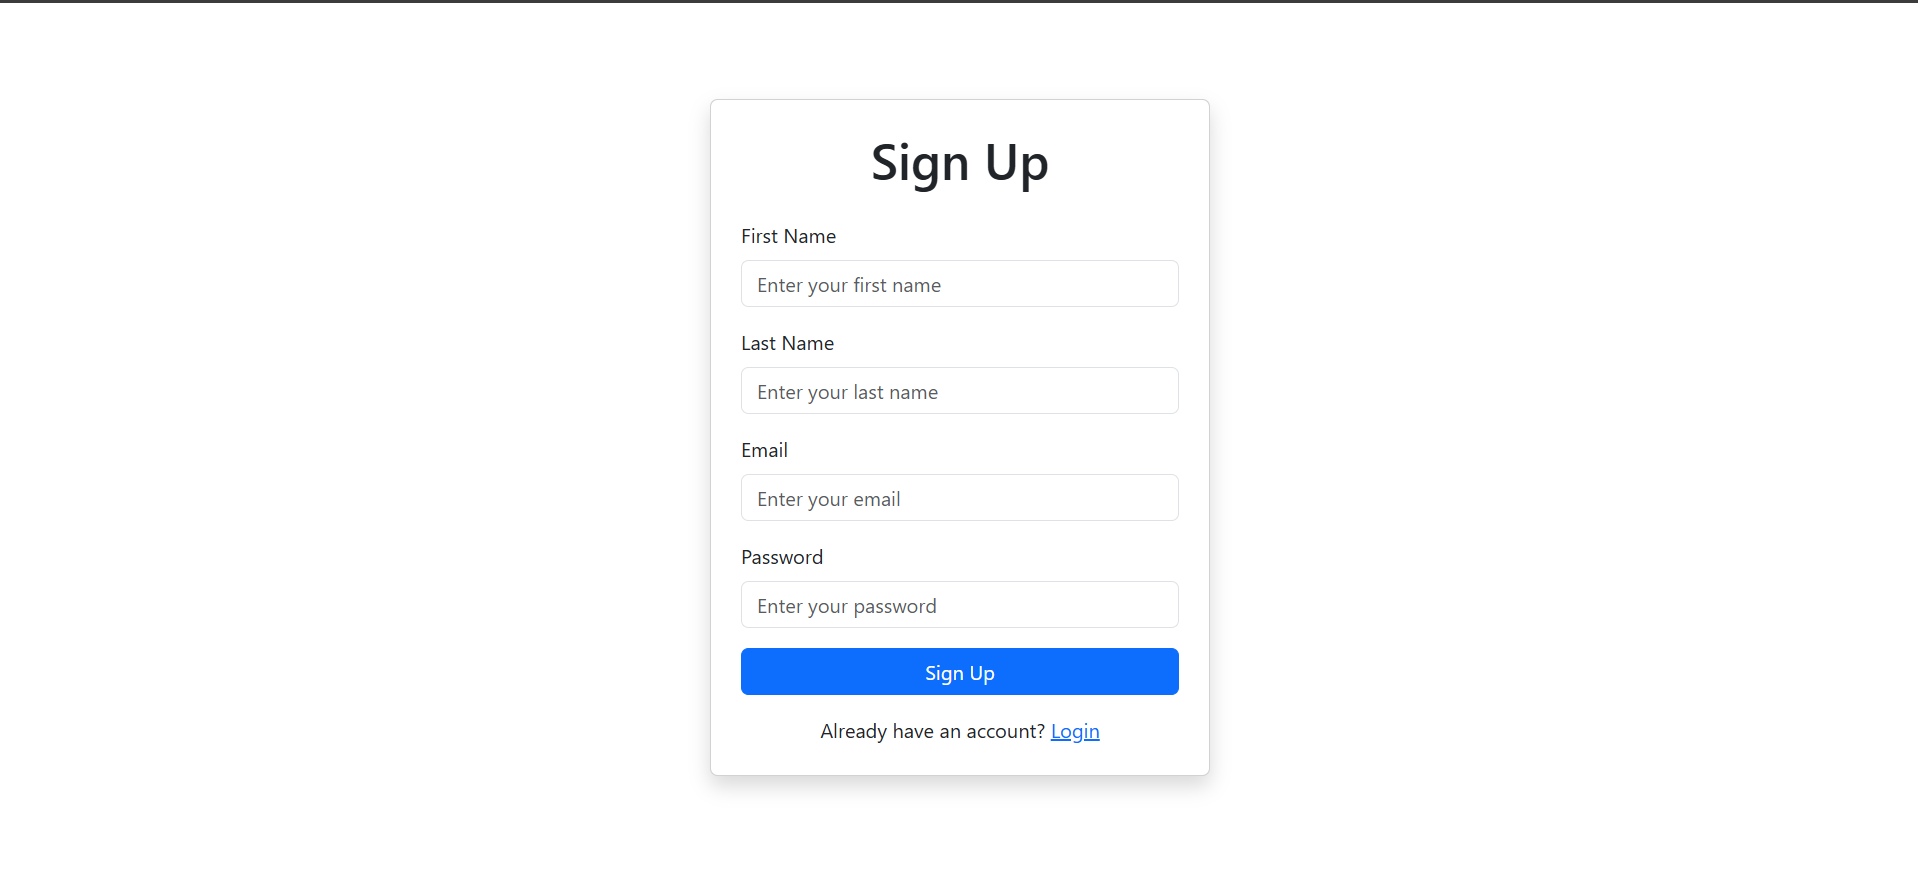
\includegraphics[width=\textwidth]{./UI_images/signup.png}
  \caption{Sign-up Page}
  \label{fig:auth_page}
\end{figure}

\begin{figure}[H]
  \centering
  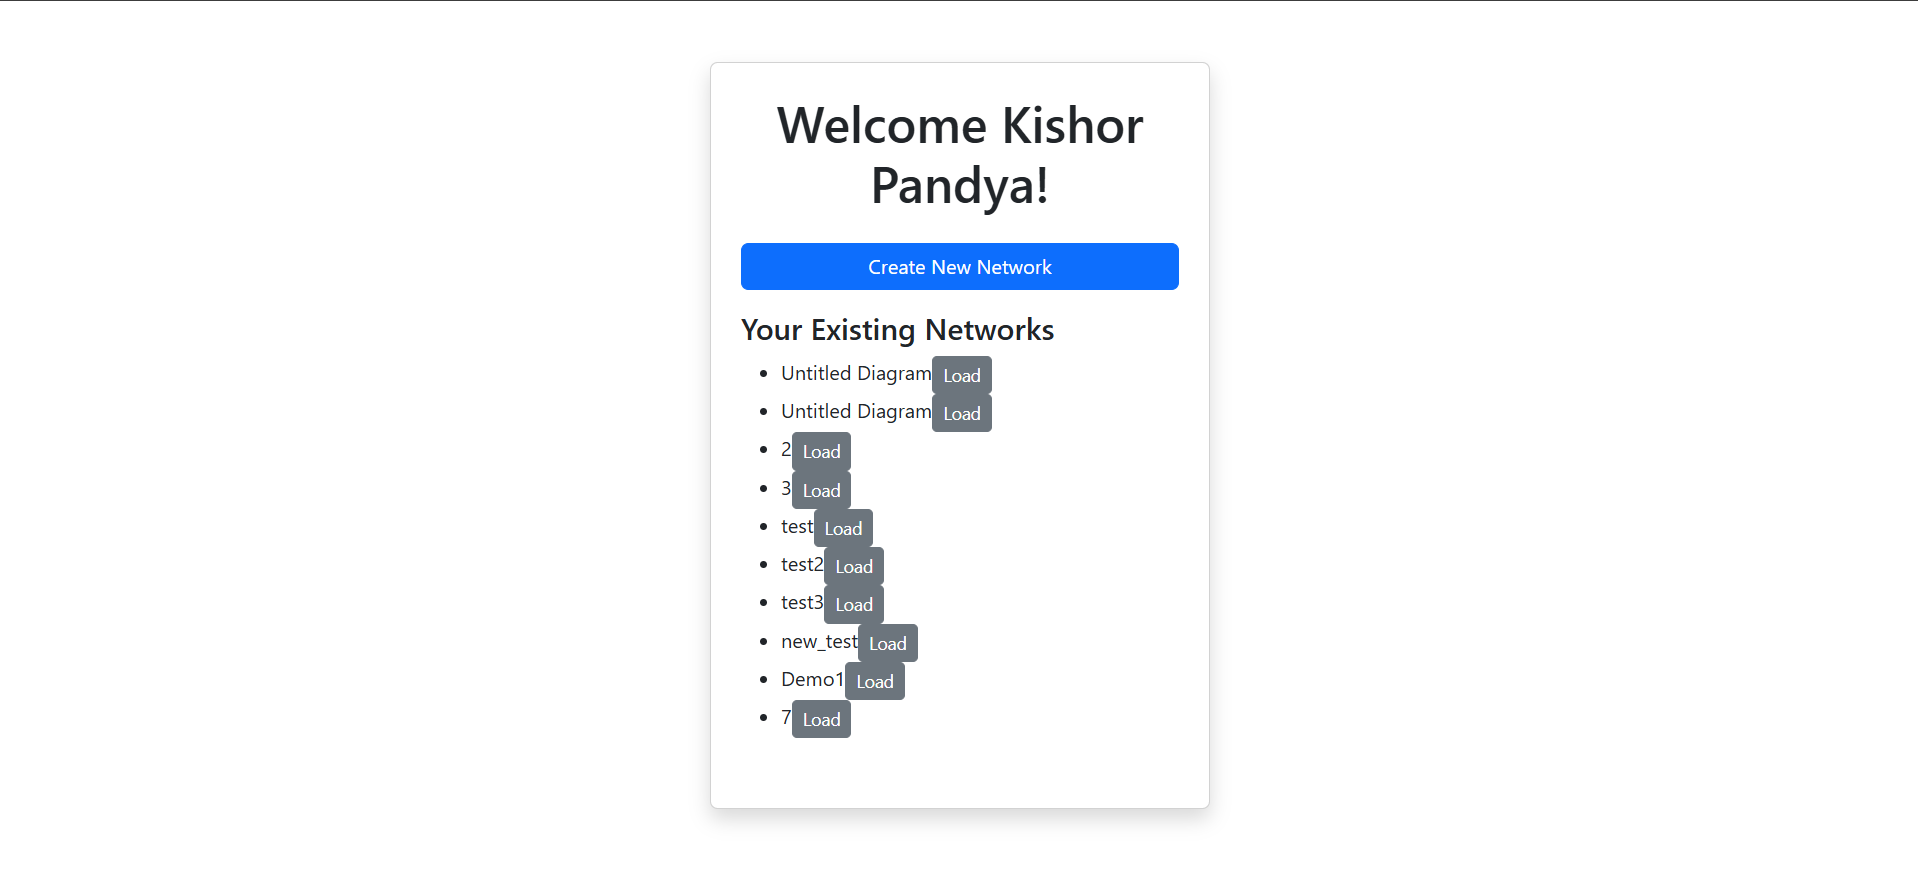
\includegraphics[width=\textwidth]{./UI_images/Dashboard1.png}
  \caption{Dashboard Page}
  \label{fig:auth_page}
\end{figure}

\begin{figure}[H]
  \centering
  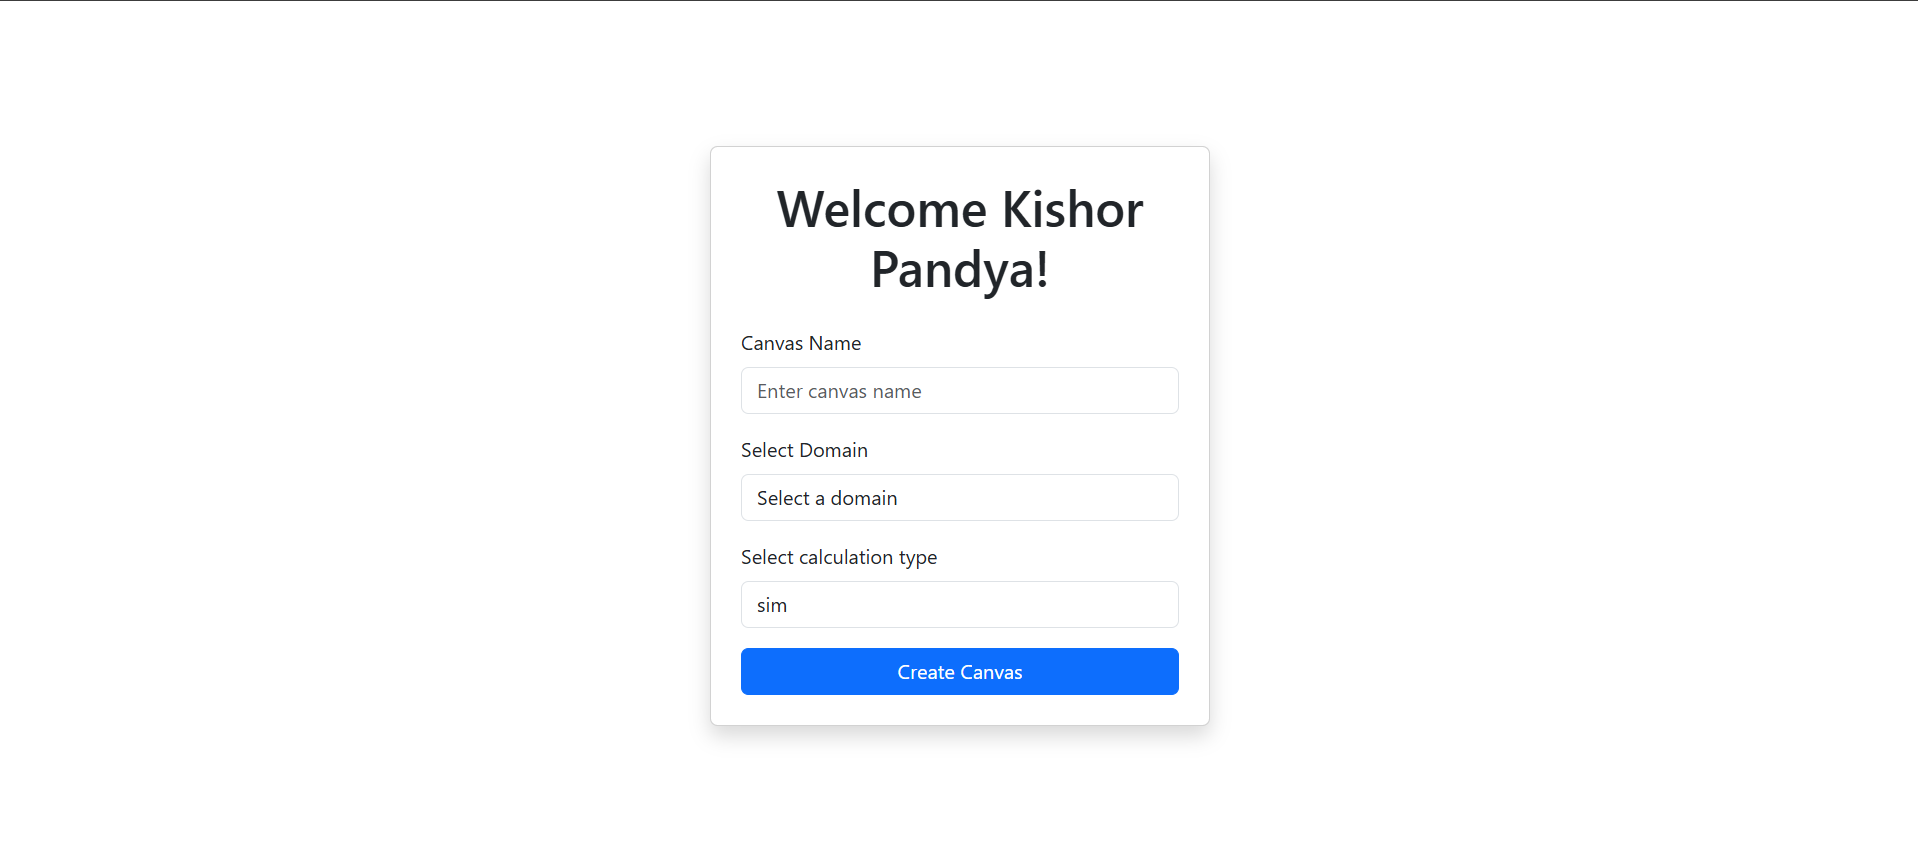
\includegraphics[width=\textwidth]{./UI_images/Dashboard2.png}
  \caption{Dashboard Page, when create is clicked}
  \label{fig:auth_page}
\end{figure}

\begin{figure}[H]
  \centering
  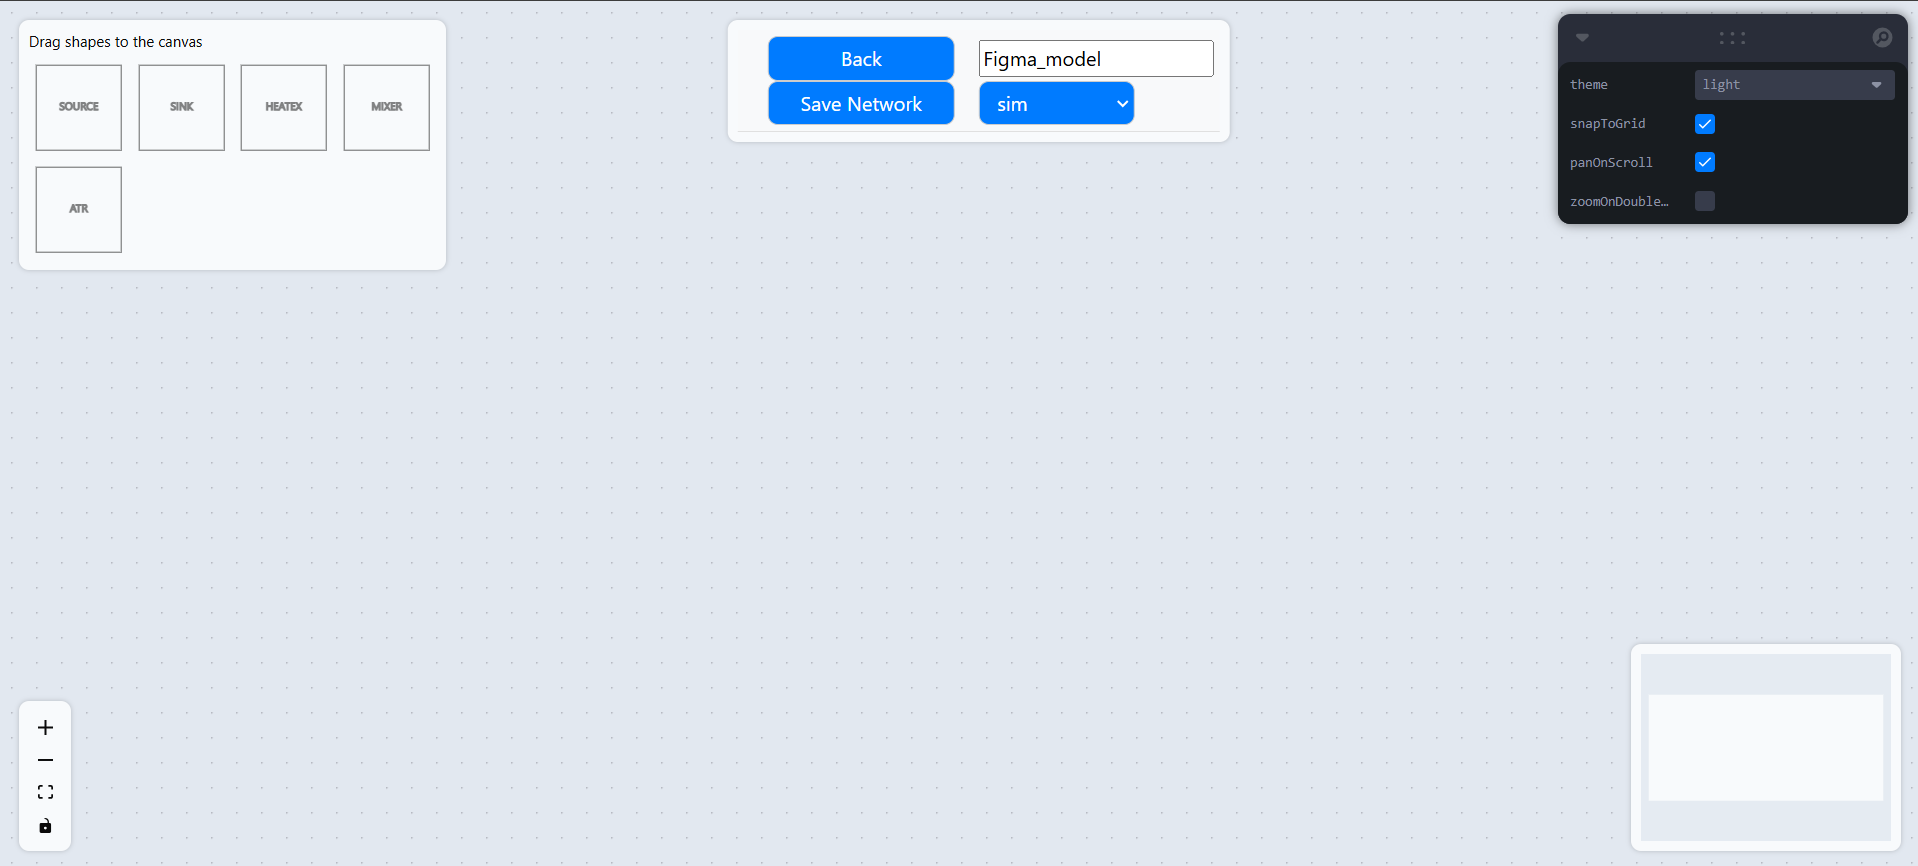
\includegraphics[width=\textwidth]{./UI_images/Canvas.png}
  \caption{Canvas Page}
  \label{fig:auth_page}
\end{figure}

\begin{figure}[H]
  \centering
  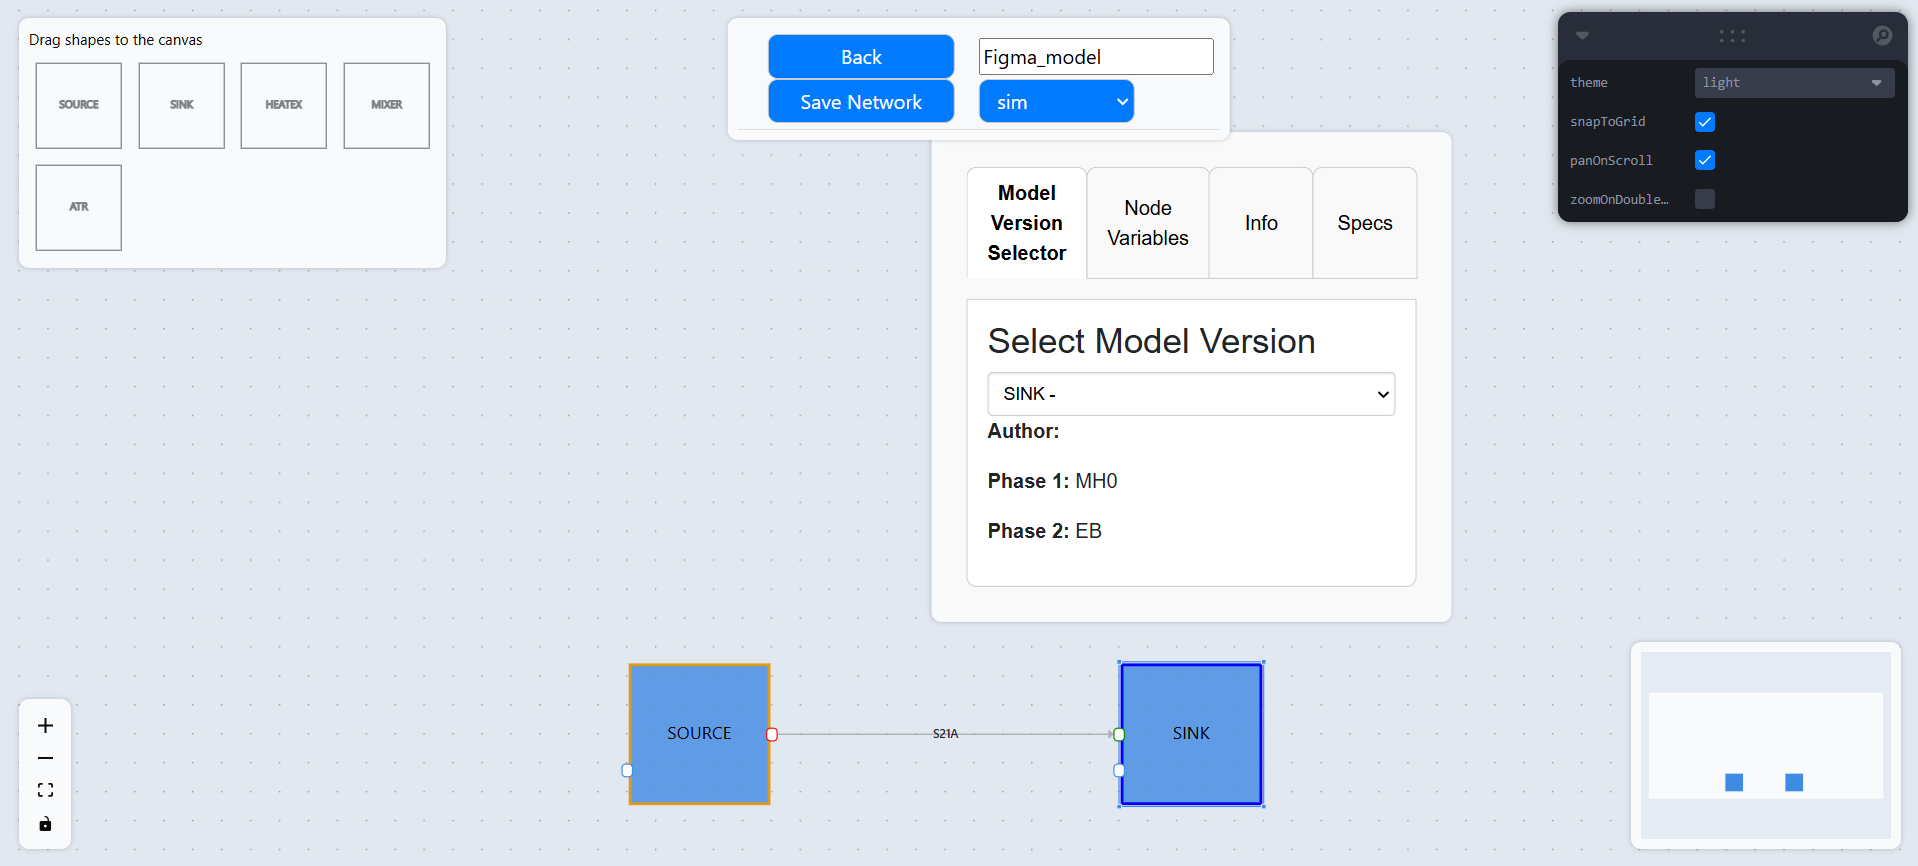
\includegraphics[width=\textwidth]{./UI_images/Canvas_inuse.png}
  \caption{Canvas Page when in use}
  \label{fig:auth_page}
\end{figure}

\bibliographystyle {plainnat}
\bibliography{../../../refs/References}

\newpage{}

\end{document}
